\documentclass[11pt]{article}
\usepackage{listings}
\usepackage{tikz}
\usepackage{url}
\usepackage{hyperref}
%\usepackage{algorithm2e}
\usetikzlibrary{arrows,automata,shapes,positioning}
\tikzstyle{block} = [rectangle, draw, fill=blue!20, 
    text width=2.5em, text centered, rounded corners, minimum height=2em]
\tikzstyle{bw} = [rectangle, draw, fill=blue!20, 
    text width=3.5em, text centered, rounded corners, minimum height=2em]

\newcommand{\handout}[5]{
  \noindent
  \begin{center}
  \framebox{
    \vbox{
      \hbox to 5.78in { {\bf ECE459: Programming for Performance } \hfill #2 }
      \vspace{4mm}
      \hbox to 5.78in { {\Large \hfill #5  \hfill} }
      \vspace{2mm}
      \hbox to 5.78in { {\em #3 \hfill #4} }
    }
  }
  \end{center}
  \vspace*{4mm}
}

\lstset{basicstyle=\ttfamily \scriptsize}

\newcommand{\lecture}[4]{\handout{#1}{#2}{#3}{#4}{Lecture #1}}
\topmargin 0pt
\advance \topmargin by -\headheight
\advance \topmargin by -\headsep
\textheight 8.9in
\oddsidemargin 0pt
\evensidemargin \oddsidemargin
\marginparwidth 0.5in
\textwidth 6.5in

\parindent 0in
\parskip 1.5ex
%\renewcommand{\baselinestretch}{1.25}

\begin{document}

\lecture{6 --- January 16, 2015}{Winter 2015}{Patrick Lam}{version 1}

\section*{Assignment 1 Discussion}
We talked about how to do assignment 1. The task is to reassemble a
picture that you fetch over the Internet using curl. You get a C
implementation that uses curl to fetch the code over the network and
uses libpng to read and write PNG files. It populates a buffer based
on the input files and outputs a buffer combining the files'
content.

\paragraph{Main Loop.} The main loop looks like this:
\begin{tabbing}
\=   main loop: until all image fragment fetched,\\
\> ~~~~ \=  retrieve the fragment over the network;\\
\> \>  copy bits into our array;\\
\> Then, write all the bits in one PNG file.
\end{tabbing}

You hand in (0) a fix to a resource leak in my code; (1) a pthread
parallelized implementation; (2) a nonblocking I/O implementation
using the libcurl multi-handle interface; and (3) an Amdahl's Law
etc. discussion.

\paragraph{Retrieving the files.} I discussed the API for retrieving
the file:

\begin{lstlisting}
  curl_easy_setopt(curl, CURLOPT_URL, url);

  // do curl request; check for errors
  res = curl_easy_perform(curl);
\end{lstlisting}

(The server then gives you back an arbitrary image fragment and you
have to loop util you get them all.) However, that wasn't
enough. Before that, I had to tell curl where to put the file---it was
to use the {\tt write\_cb} callback function.

    \begin{lstlisting}
  struct bufdata bd; 
  bd.buf = input_buffer; 
  curl_easy_setopt(curl, CURLOPT_WRITEFUNCTION, write_cb);
  curl_easy_setopt(curl, CURLOPT_WRITEDATA, &bd);
    \end{lstlisting}

{\tt write\_cb} puts data in {\tt input\_buffer} using a straightforward {\tt
  memcpy}-based implementation. It doesn't do anything fancy, but does
make sure that it doesn't overflow the buffer.

\paragraph{Parsing the input .PNG files.} This consisted of a
bunch of {\tt libpng} magic: {\tt libpng} will put the image data
in a {\tt png\_bytep *} array, where each element points to a row of
pixels.

My {\tt read\_png\_file} function allocates the data. I've
chosen the convention that the caller must free the returned value.
These conventions can trip you up and cause memory leaks if they
aren't inconsistently used. 

Afterwards, {\tt paint\_destination} fills in the output array, pasting together
the fragments.

\paragraph{Writing the output .PNG file.} This is simply symmetric
to the read part.

Note: be sure to free everything! (We'll check.)

\subsection*{Using pthreads}
I found this to be quite easy, but I noticed that people found all sorts
of ways to do this which I hadn't anticipated. In any case, I expect that
you will have to do some refactoring. I sort of on purpose made it not
immediately amenable to refactoring.

You need to start some threads. Then, justify why the threads are not
interfering. Time the result.

\subsection*{Nonblocking I/O}
This part is more complicated than using threads. It is typically lower
overhead (why?) and good for servers which handle lots of connections.
But it is also more of a pain to program. On the other hand, you don't have
to worry about shared state.

\paragraph{JavaScript option.} 
As an alternate option, you were allowed to use either {\tt node.js}
or client-side JavaScript to do the nonblocking I/O. You are on your
own for this option. Let me know; I'll mark those solutions myself.

\section*{Asynchronous/non-blocking I/O}

Let's start with some juicy quotes.

\begin{center}
  \fbox{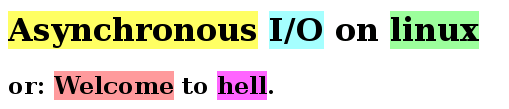
\includegraphics[width=.7\textwidth]{L06/aio-linux.png}}\\
{\scriptsize (mirrored at \url{compgeom.com/~piyush/teach/4531_06/project/hell.html})}
   \\[2em]

   ``Asynchronous I/O, for example, is often infuriating.''\\
\hfill --- Robert Love. {\em Linux System Programming, 2nd ed, } page 215.

\end{center}

To motivate the need for non-blocking I/O, consider some standard I/O code:

\begin{lstlisting}
    fd = open(...);
    read(...);
    close(fd);
\end{lstlisting}

This isn't very performant. The problem is that the {\tt read} call will
{\em block}. So, your program doesn't get to use the zillions of CPU cycles that
are happening while the I/O operation is occurring.

\paragraph{As seen previously: threads.} That can be fine if
you have some other code running to do work---for instance, other threads
do a good job mitigating the I/O latency, perhaps doing I/O themselves.
But maybe you would rather not use threads. Why not?

\begin{itemize}
\item potential race conditions;
\item overhead due to per-thread stacks; or
\item limitations due to maximum numbers of threads.
\end{itemize}

\paragraph{Live coding example.} To illustrate the max-threads
issue, we wrote {\tt threadbomb.c}, which explored how many simultaneous threads
one could start on my computer.

\paragraph{Non-blocking I/O.} The main point of this lecture, though,
is non-blocking/asynchronous I/O. The simplest example:

\begin{lstlisting}
    fd = open(..., O_NONBLOCK);
    read(...); // returns instantly!
    close(fd);
\end{lstlisting}

In principle, the {\tt read} call is supposed to return instantly,
whether or not results are ready. That was easy!

Well, not so much. The {\tt O\_NONBLOCK} flag actually only has the
desired behaviour on sockets. The semantics of {\tt O\_NONBLOCK} is
for I/O calls to not block, in the sense that they should never wait
for data while there is no data available.

Unfortunately, files always have data available. Under Linux, you'd have
to use {\tt aio} calls to be able to send requests to the I/O subsystem
asynchronously and not, for instance, wait for the disk to spin up.
We won't talk about them, but they operate along the same lines as what
we will see. They just have a different API.

\end{document}
